%\chapter{Proof: Existence and uniqueness of solutions}
%\label{Proof:ExistenceUniqueness}




\chapter{Gronwall-inequality}
\label{Gronwall}
\begin{lemma}[Gronwall-inequality]
Let \(\phi\) and f be nonnegative and continuous functions defined on [0,T]. Let $C>0$ denote a constant. If:
\[\phi(t)\leq C + \int_0^t \! f(s)\phi(s)\,\mathrm{d}s\quad\text{for all}\:\:t\in[0,T]\]
then:
\[\phi(t)\leq C\cdot\exp(\int_0^t \! f(s)\,\mathrm{d}s) \quad\text{for all}\:\:t\in[0,T].\]
\end{lemma}
\begin{proof}

Let \(\psi(t)\) be defined as:
\[
\psi(t) = C + \int_0^t \! f(s)\phi(s)\,\mathrm{d}s.
\]
Given that \(\phi(t) \leq \psi(t)\), we substitute \(\phi(t)\) with \(\psi(t)\) in the integral:
\[
\psi(t) = C + \int_0^t \! f(s)\phi(s)\,\mathrm{d}s \leq C + \int_0^t \! f(s)\psi(s)\,\mathrm{d}s.
\]
Next, consider the function \(g(t)\) defined by:
\[
g(t) = \exp\left(-\int_0^t \! f(s)\,\mathrm{d}s\right)\psi(t).
\]
We now differentiate \(g(t)\) with respect to \(t\):
\[
\frac{\mathrm{d}g(t)}{\mathrm{d}t} = \exp\left(-\int_0^t \! f(s)\,\mathrm{d}s\right)\left[f(t)\psi(t) - f(t)\psi(t) + \frac{\mathrm{d}\psi(t)}{\mathrm{d}t}\right] = \exp\left(-\int_0^t \! f(s)\,\mathrm{d}s\right)\frac{\mathrm{d}\psi(t)}{\mathrm{d}t}.
\]
Since:
\[
\frac{\mathrm{d}\psi(t)}{\mathrm{d}t} = f(t)\phi(t),
\]
we get:
\[
\frac{\mathrm{d}g(t)}{\mathrm{d}t} = \exp\left(-\int_0^t \! f(s)\,\mathrm{d}s\right)f(t)\phi(t).
\]
Integrating from \(0\) to \(t\), we have:
\[
g(t) = g(0) + \int_0^t \exp\left(-\int_0^s \! f(\tau)\,\mathrm{d}\tau\right)f(s)\phi(s)\,\mathrm{d}s.
\]
At \(t = 0\), \(g(0) = C\). Therefore:
\[
\psi(t) \leq C\exp\left(\int_0^t \! f(s)\,\mathrm{d}s\right).
\]
Finally, since \(\phi(t) \leq \psi(t)\), we obtain:
\[
\phi(t) \leq C\cdot\exp\left(\int_0^t \! f(s)\,\mathrm{d}s\right).
\]
This completes the proof.

\end{proof}

\chapter{Source code}
\label{code}
The numerical methods presented in this thesis were implemented using Python. Key libraries include \texttt{Matplotlib} for plots and \texttt{NumPy} for numerical computations.

The complete source code with additional documentation and examples is available on GitHub at: \href{https://github.com/AmrUmeri/NumericalSDE}{\texttt{https://github.com/AmrUmeri/NumericalSDE}}. The repository contains all the necessary files to replicate the results presented in this thesis and instructions on how to run the code.

 
%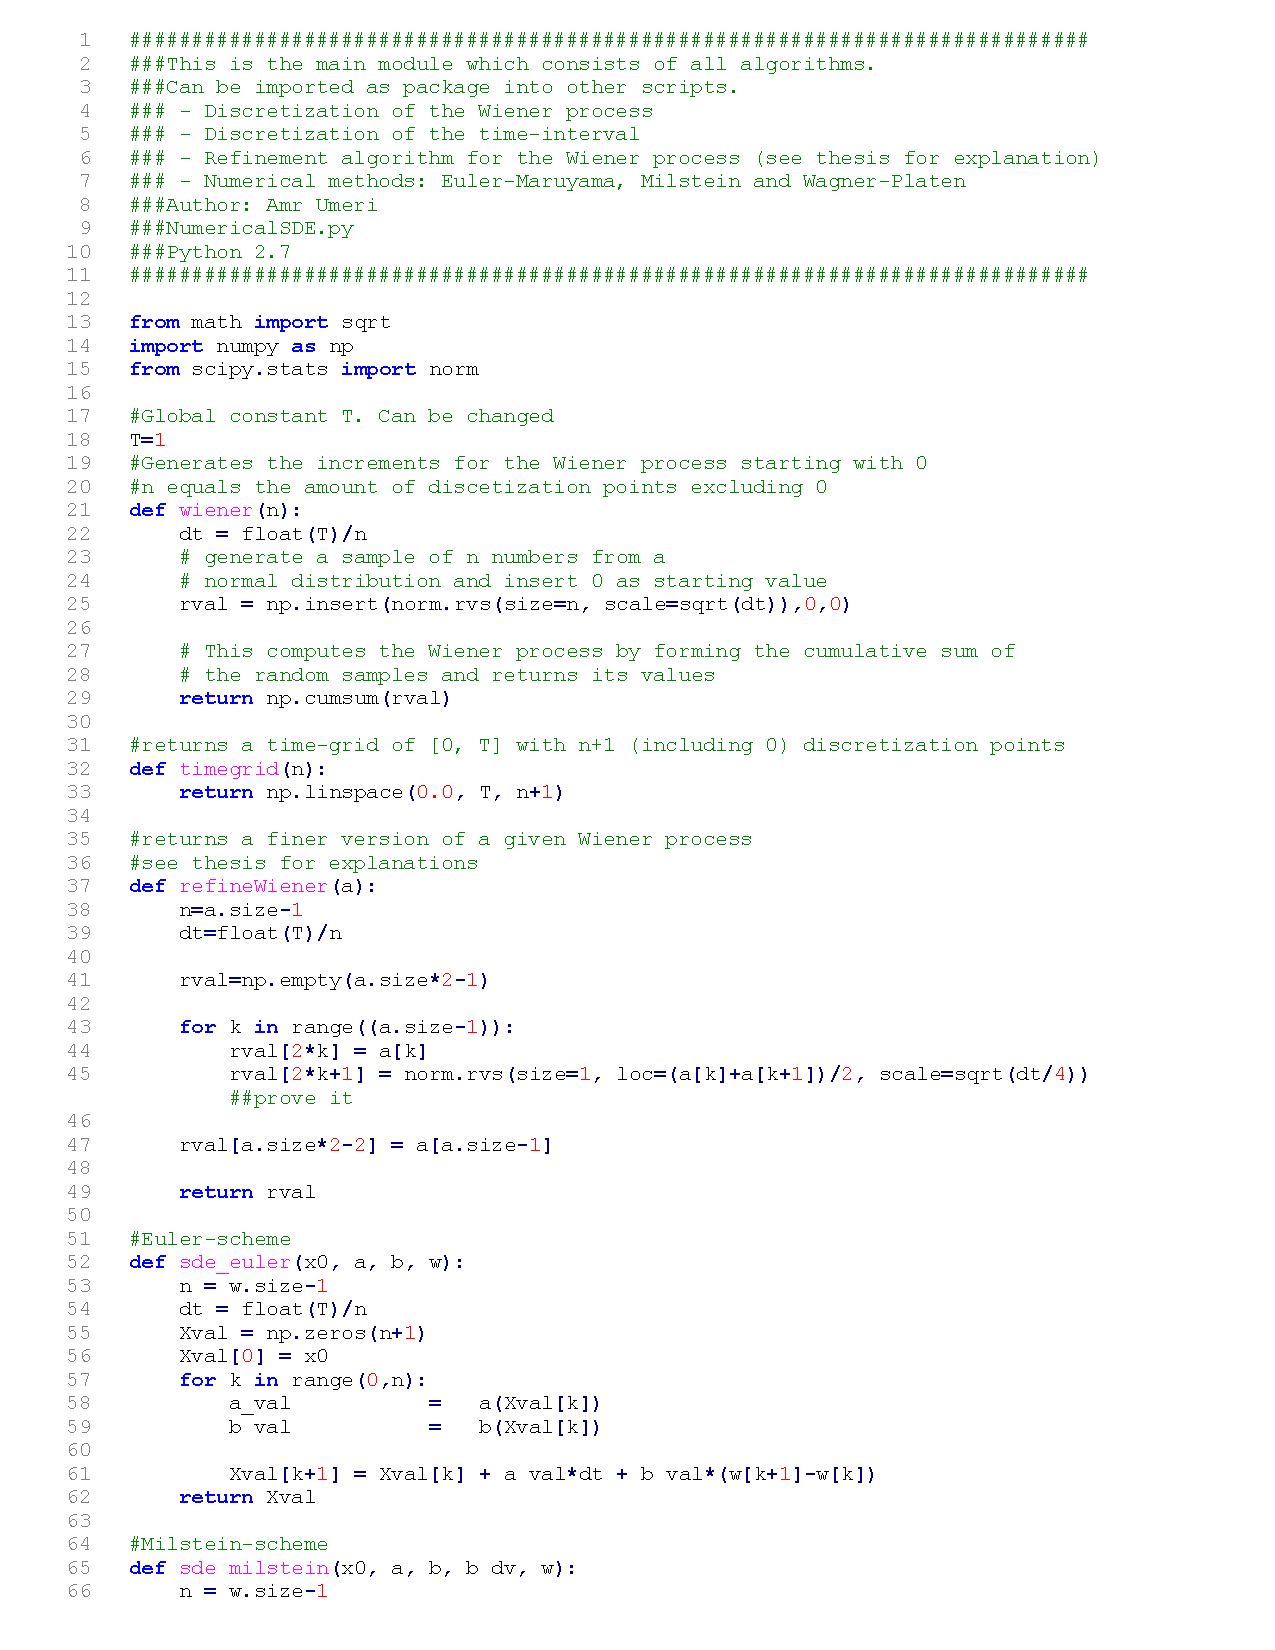
\includepdf[pages={-}]{Content/Code/NumericalSDE.pdf}
%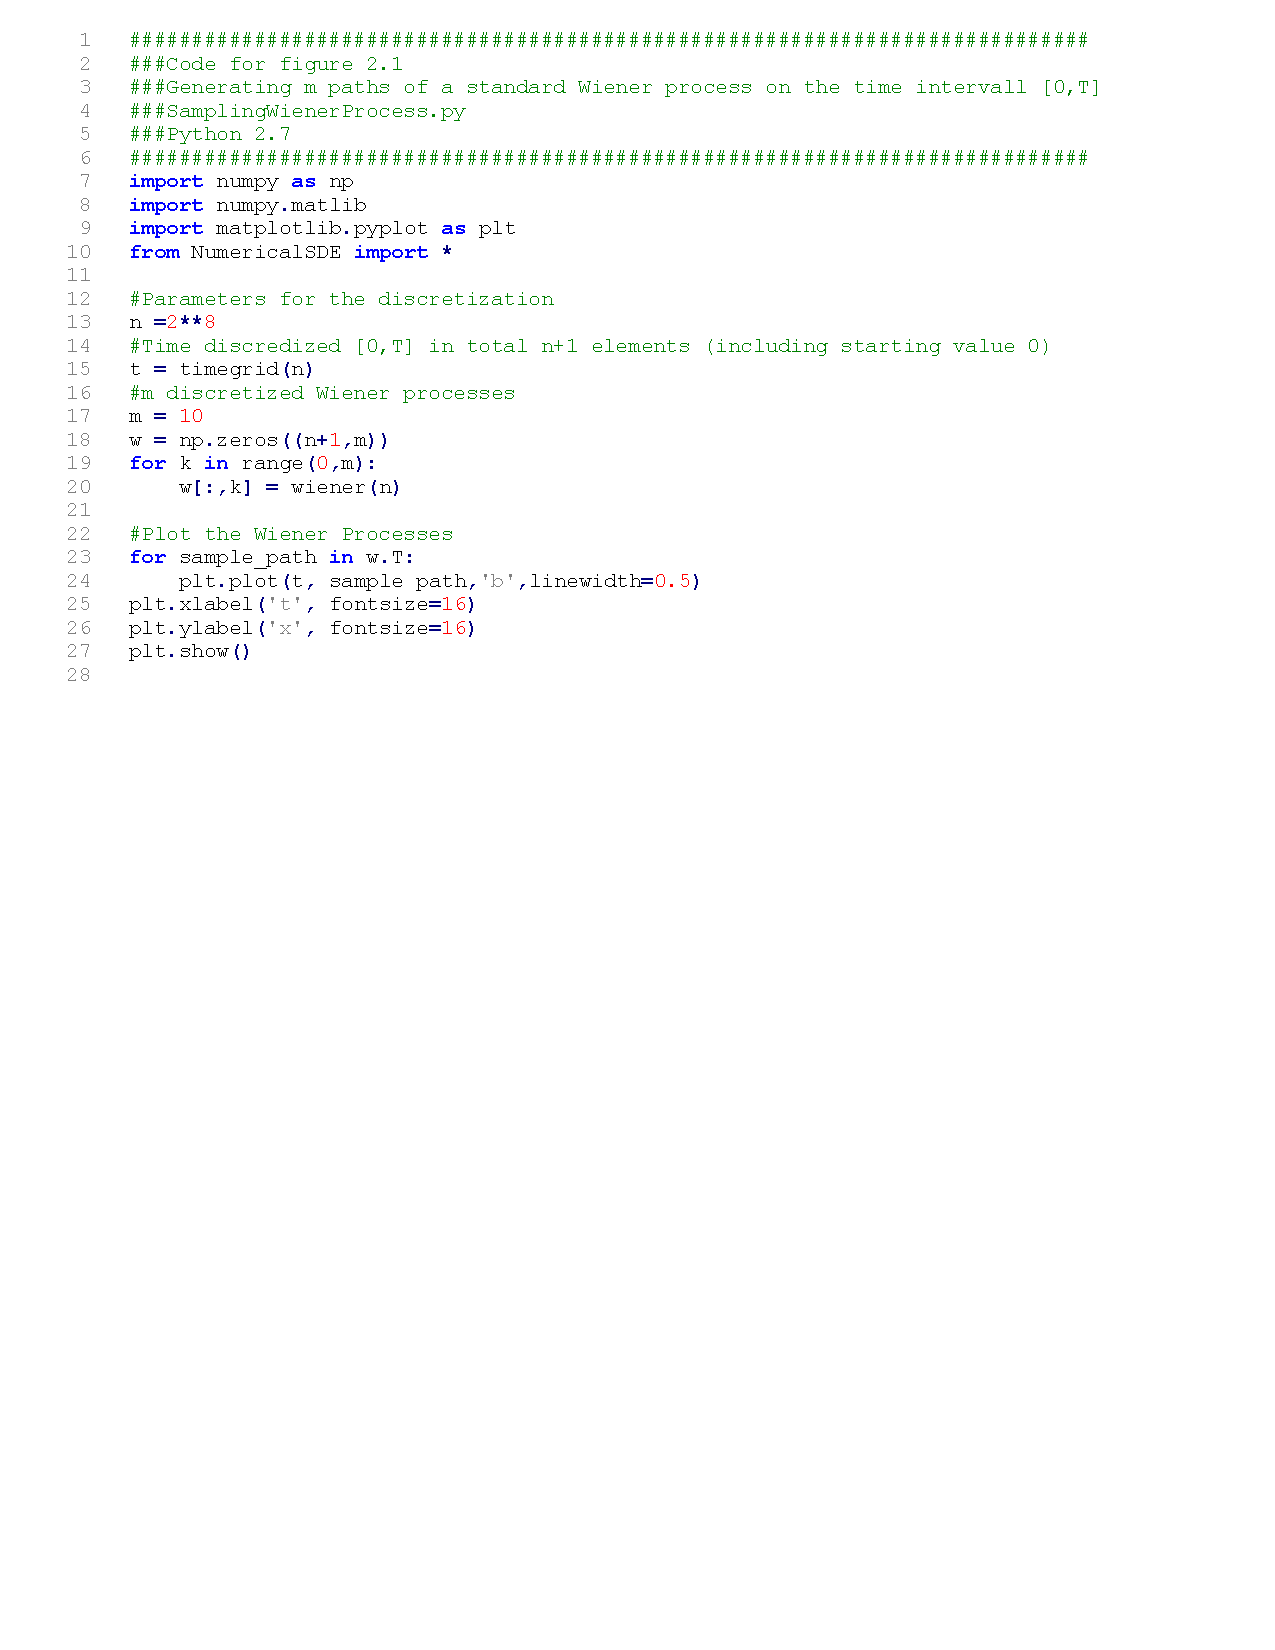
\includepdf[pages={-}]{Content/Code/SamplingWienerProcessGraphic.pdf}
%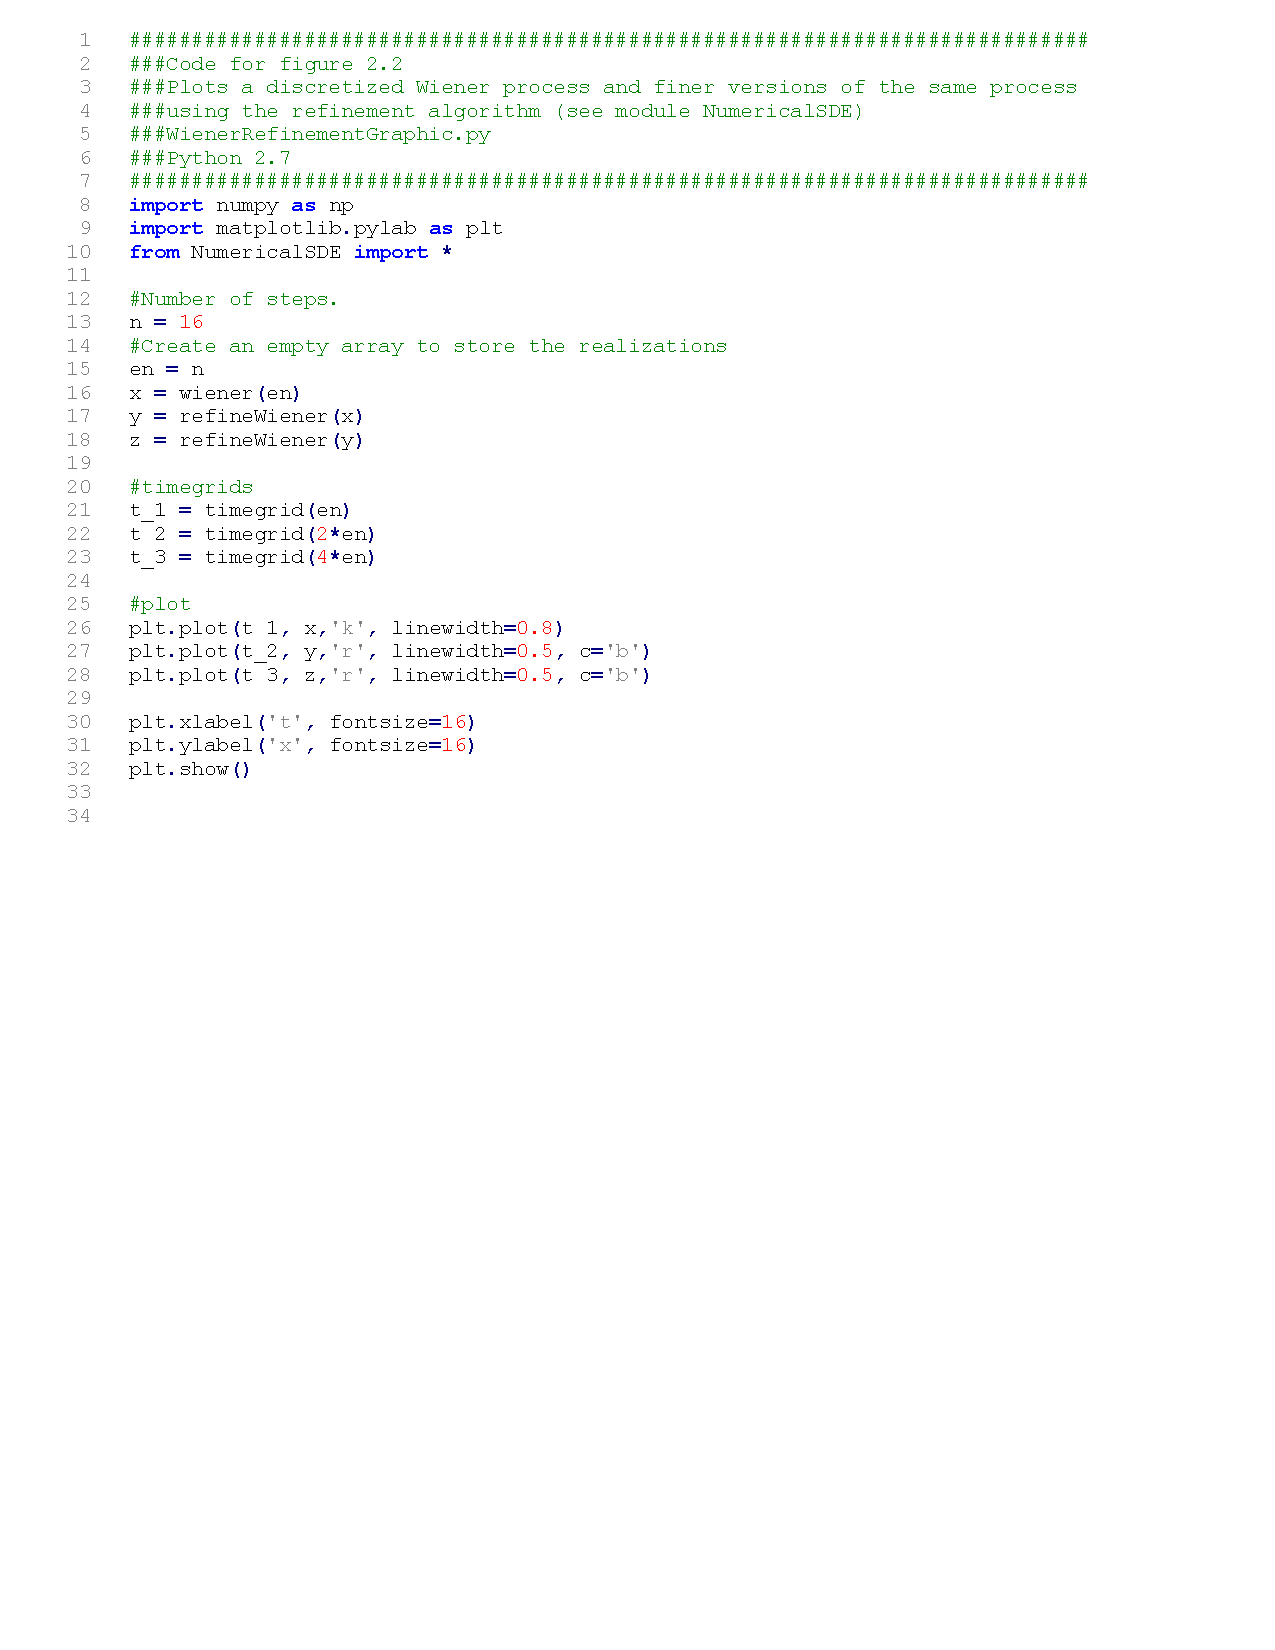
\includepdf[pages={-}]{Content/Code/WienerRefinementGraphic.pdf}
%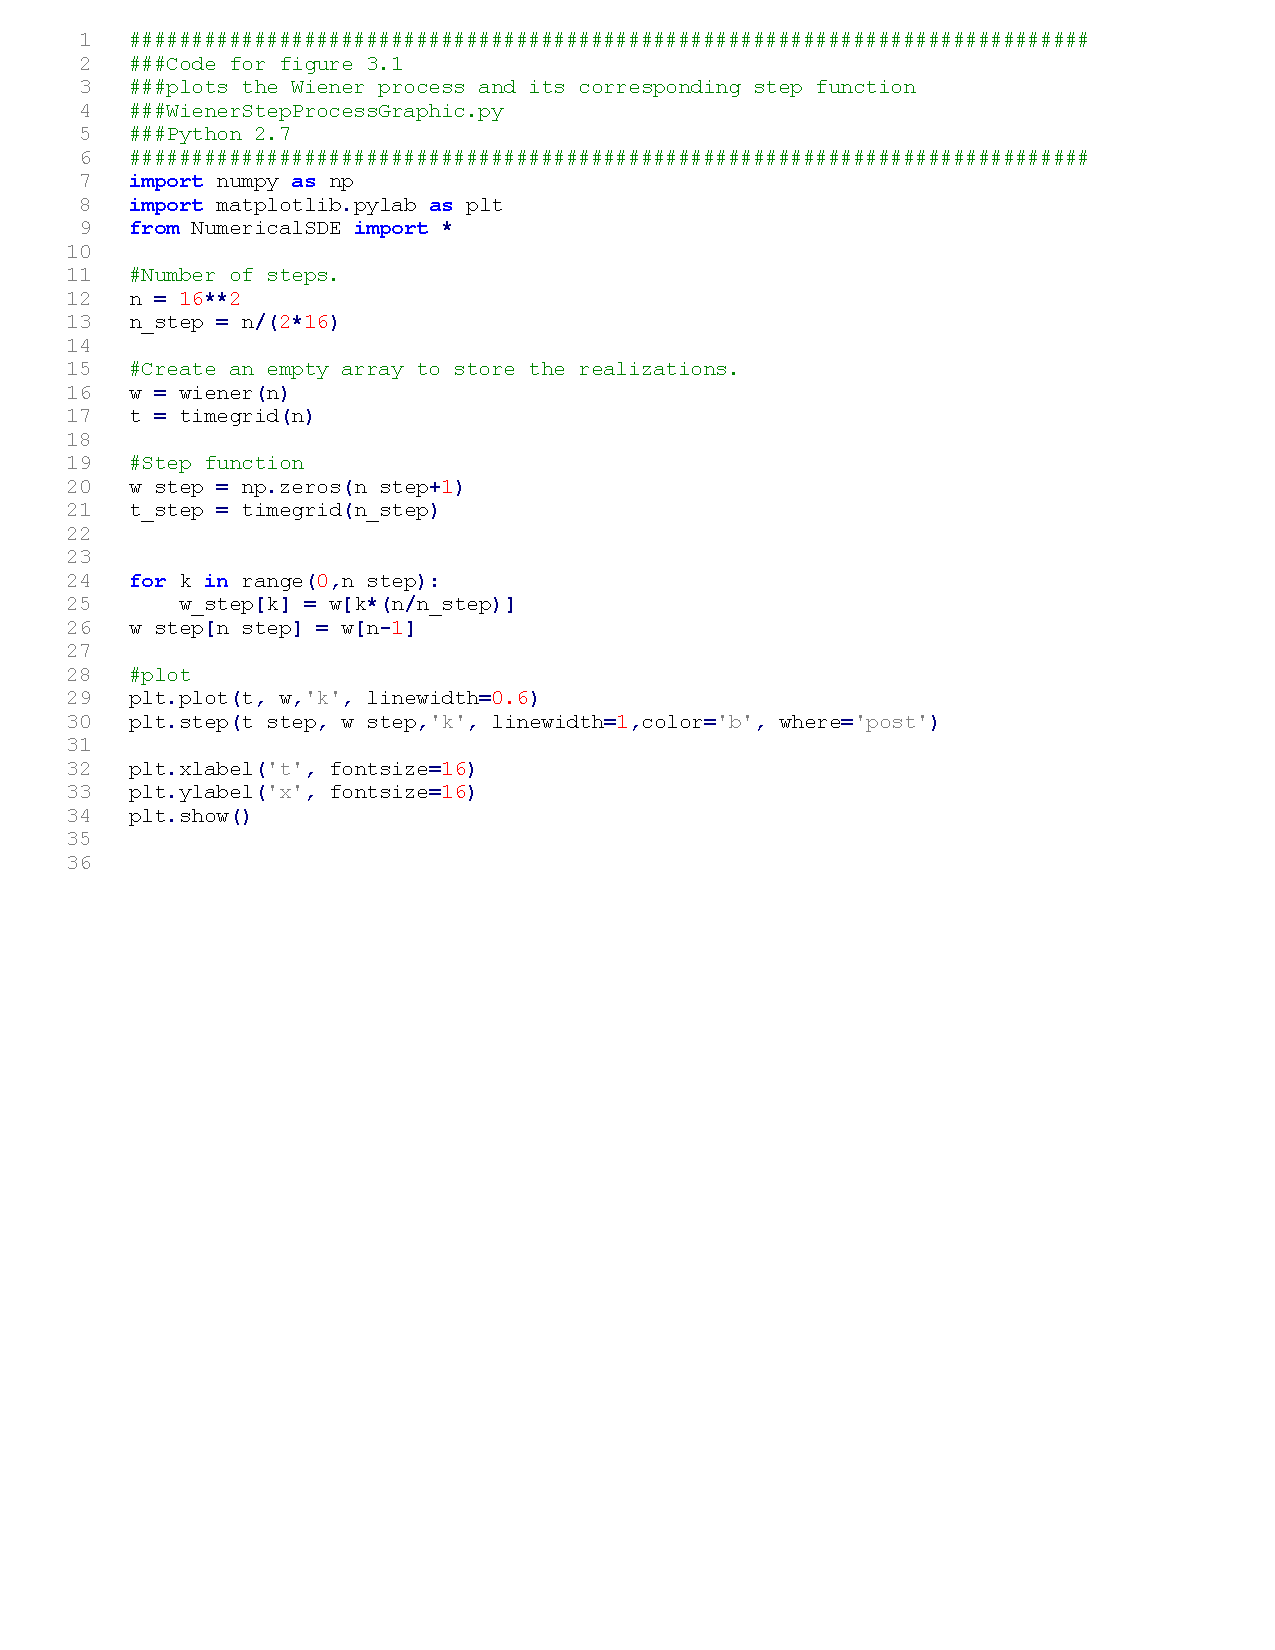
\includepdf[pages={-}]{Content/Code/WienerStepProcessGraphic.pdf}
%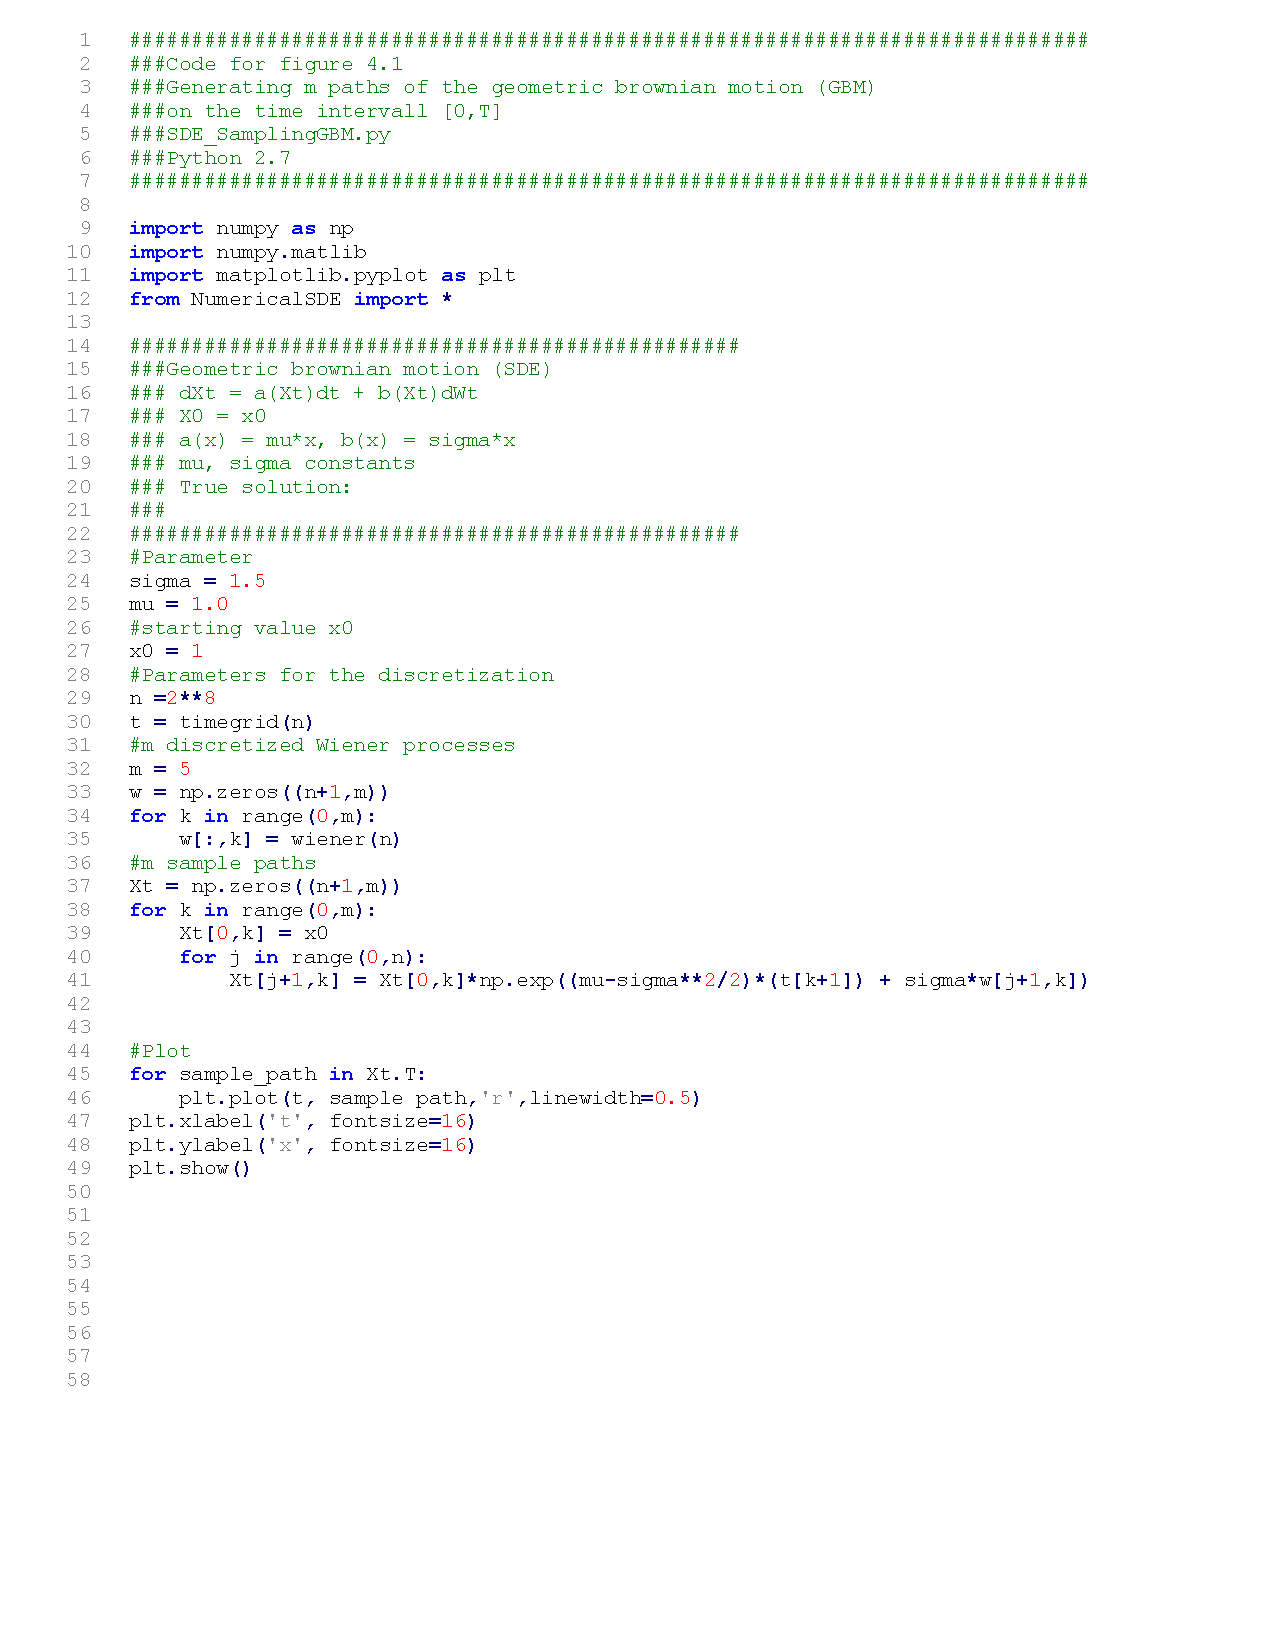
\includepdf[pages={-}]{Content/Code/SDE_SamplingGBM.pdf}
%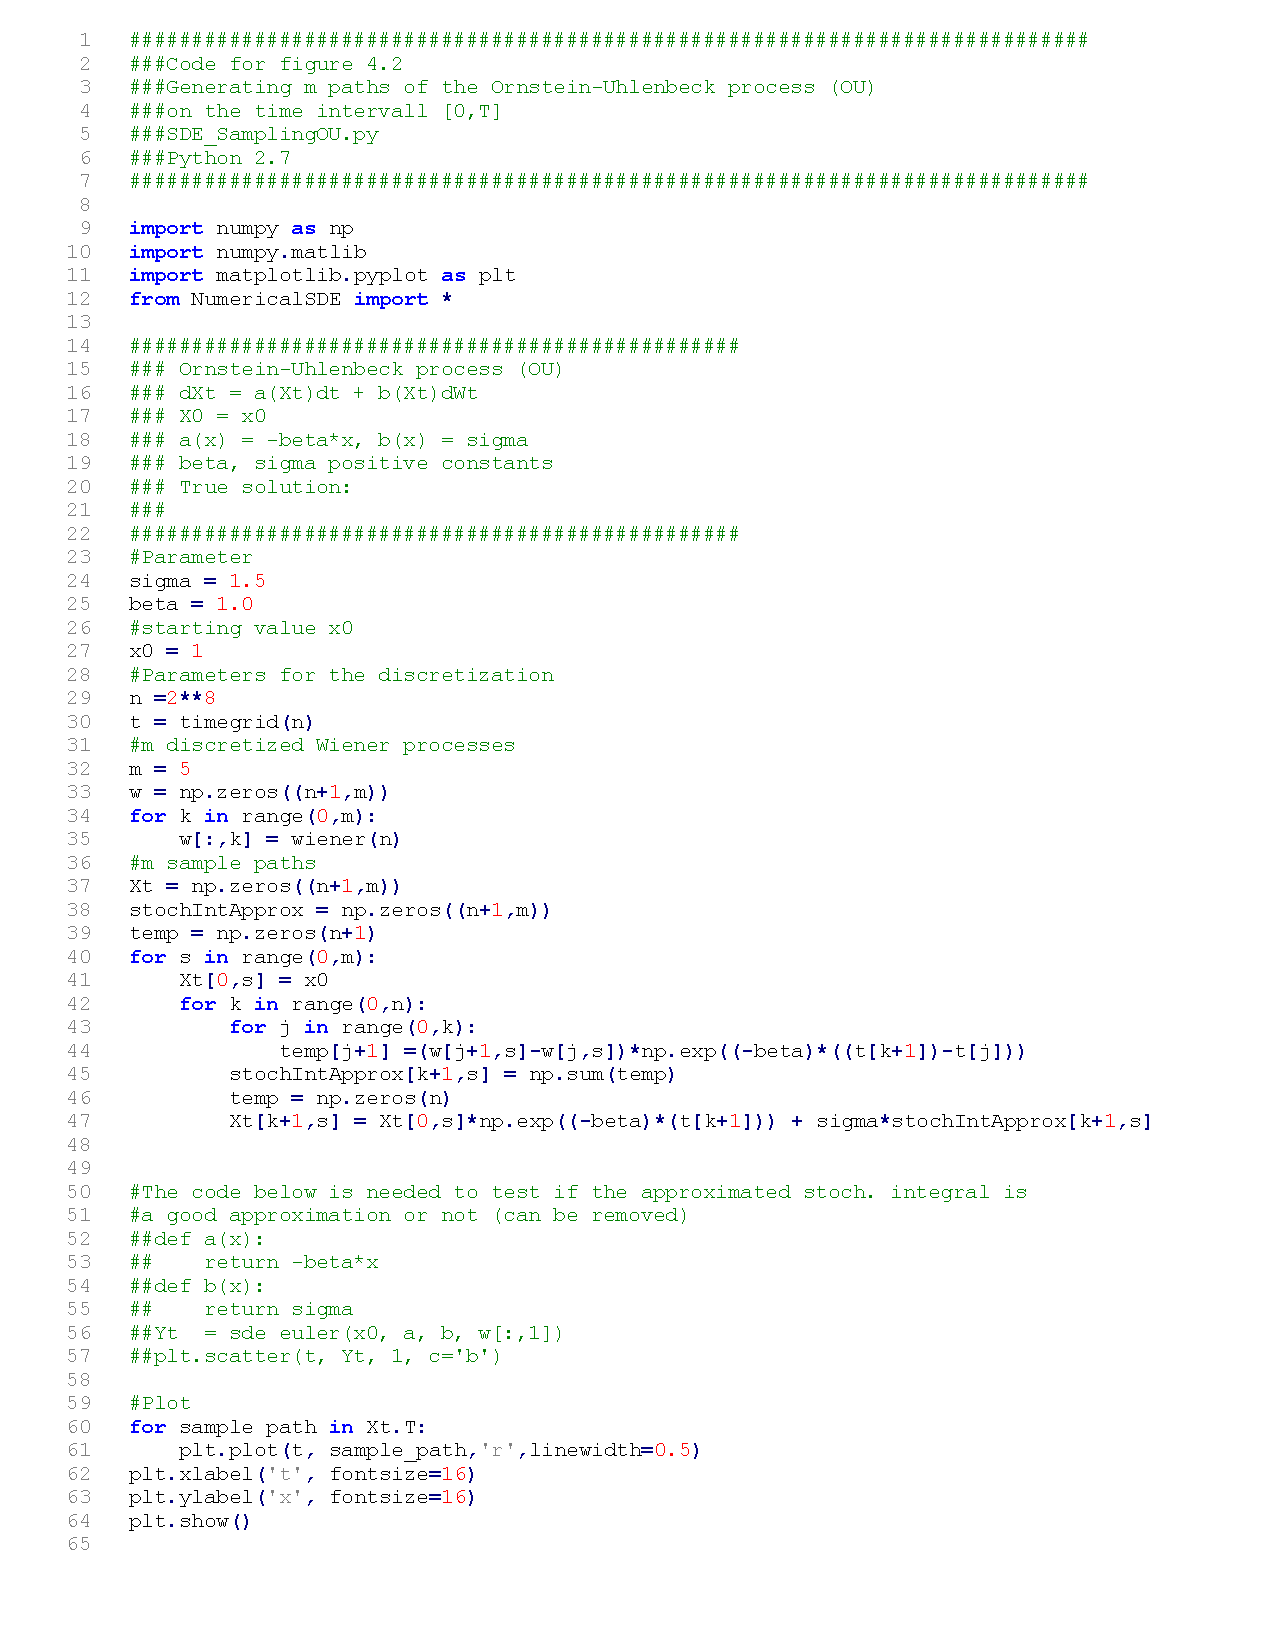
\includepdf[pages={-}]{Content/Code/SDE_SamplingOU.pdf}
%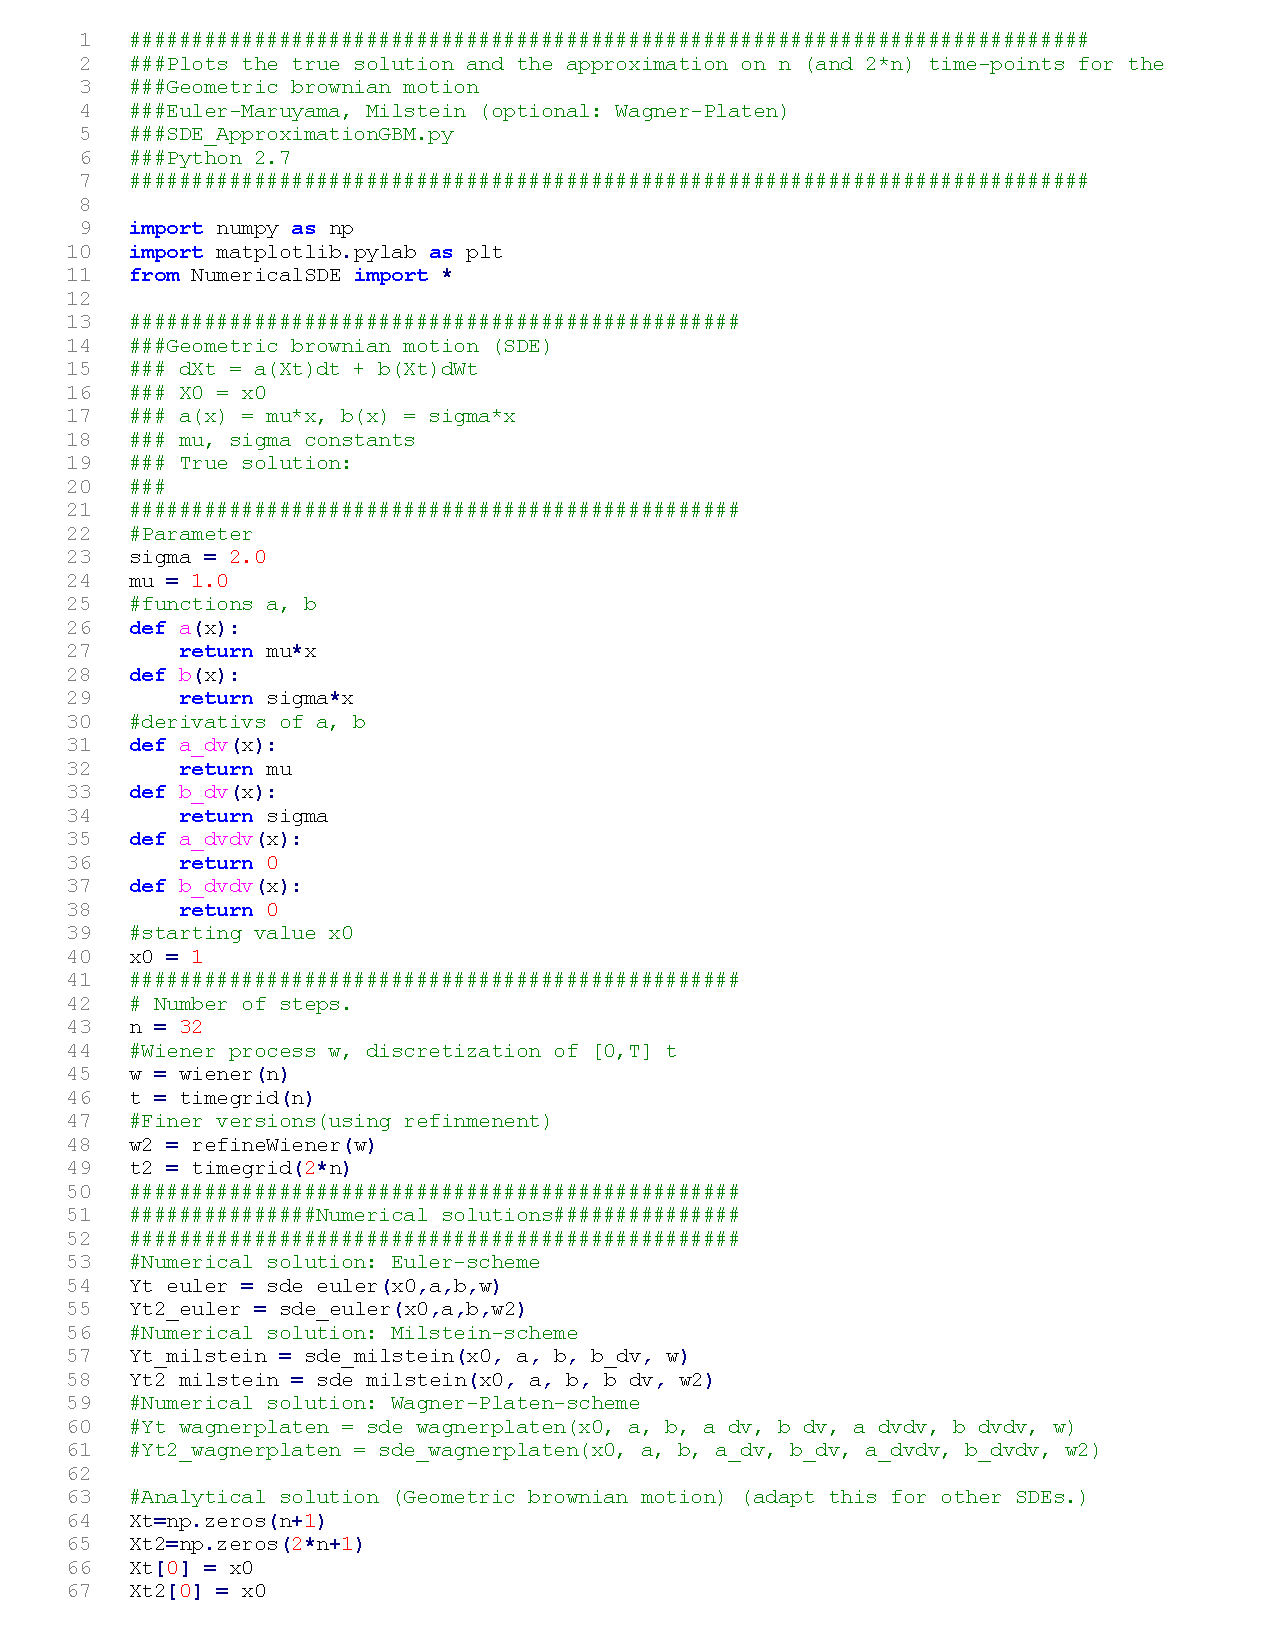
\includepdf[pages={-}]{Content/Code/SDE_ApproximationGBM.pdf}
%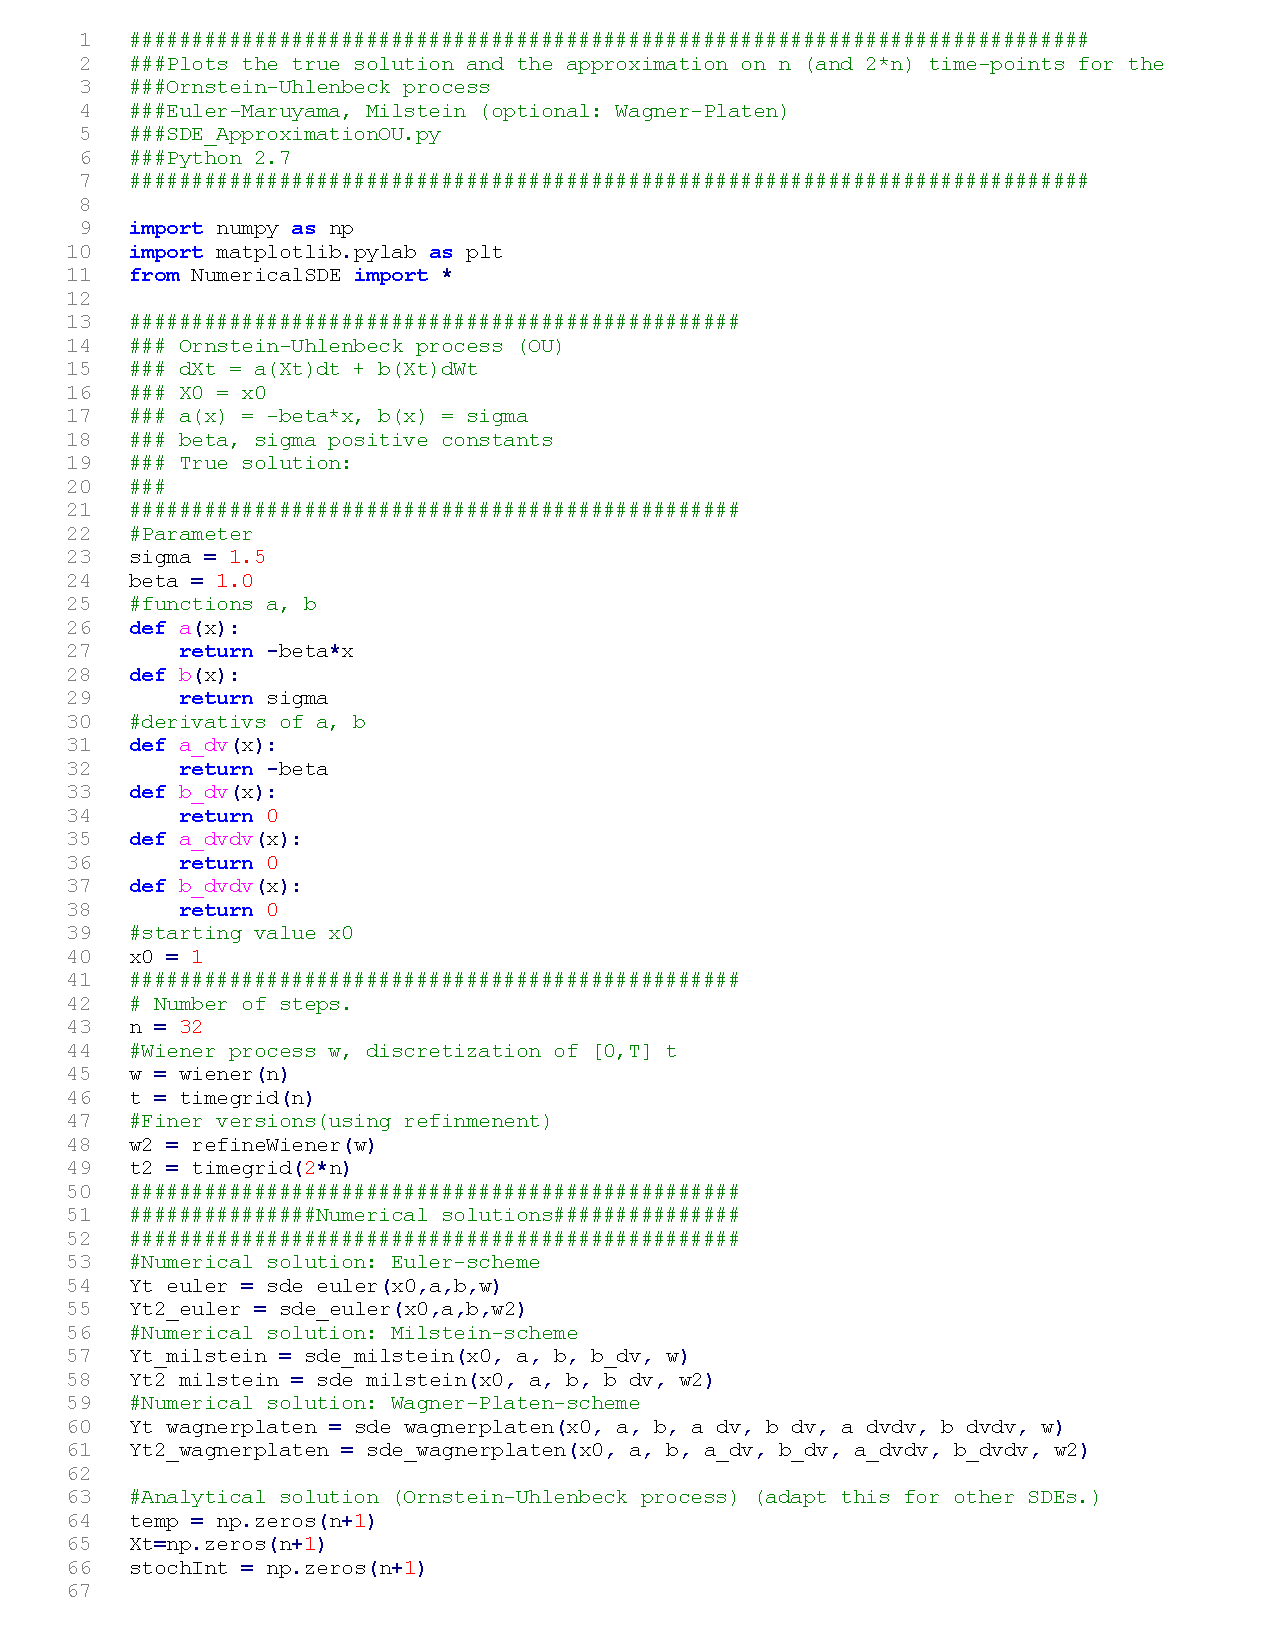
\includepdf[pages={-}]{Content/Code/SDE_ApproximationOU.pdf}
%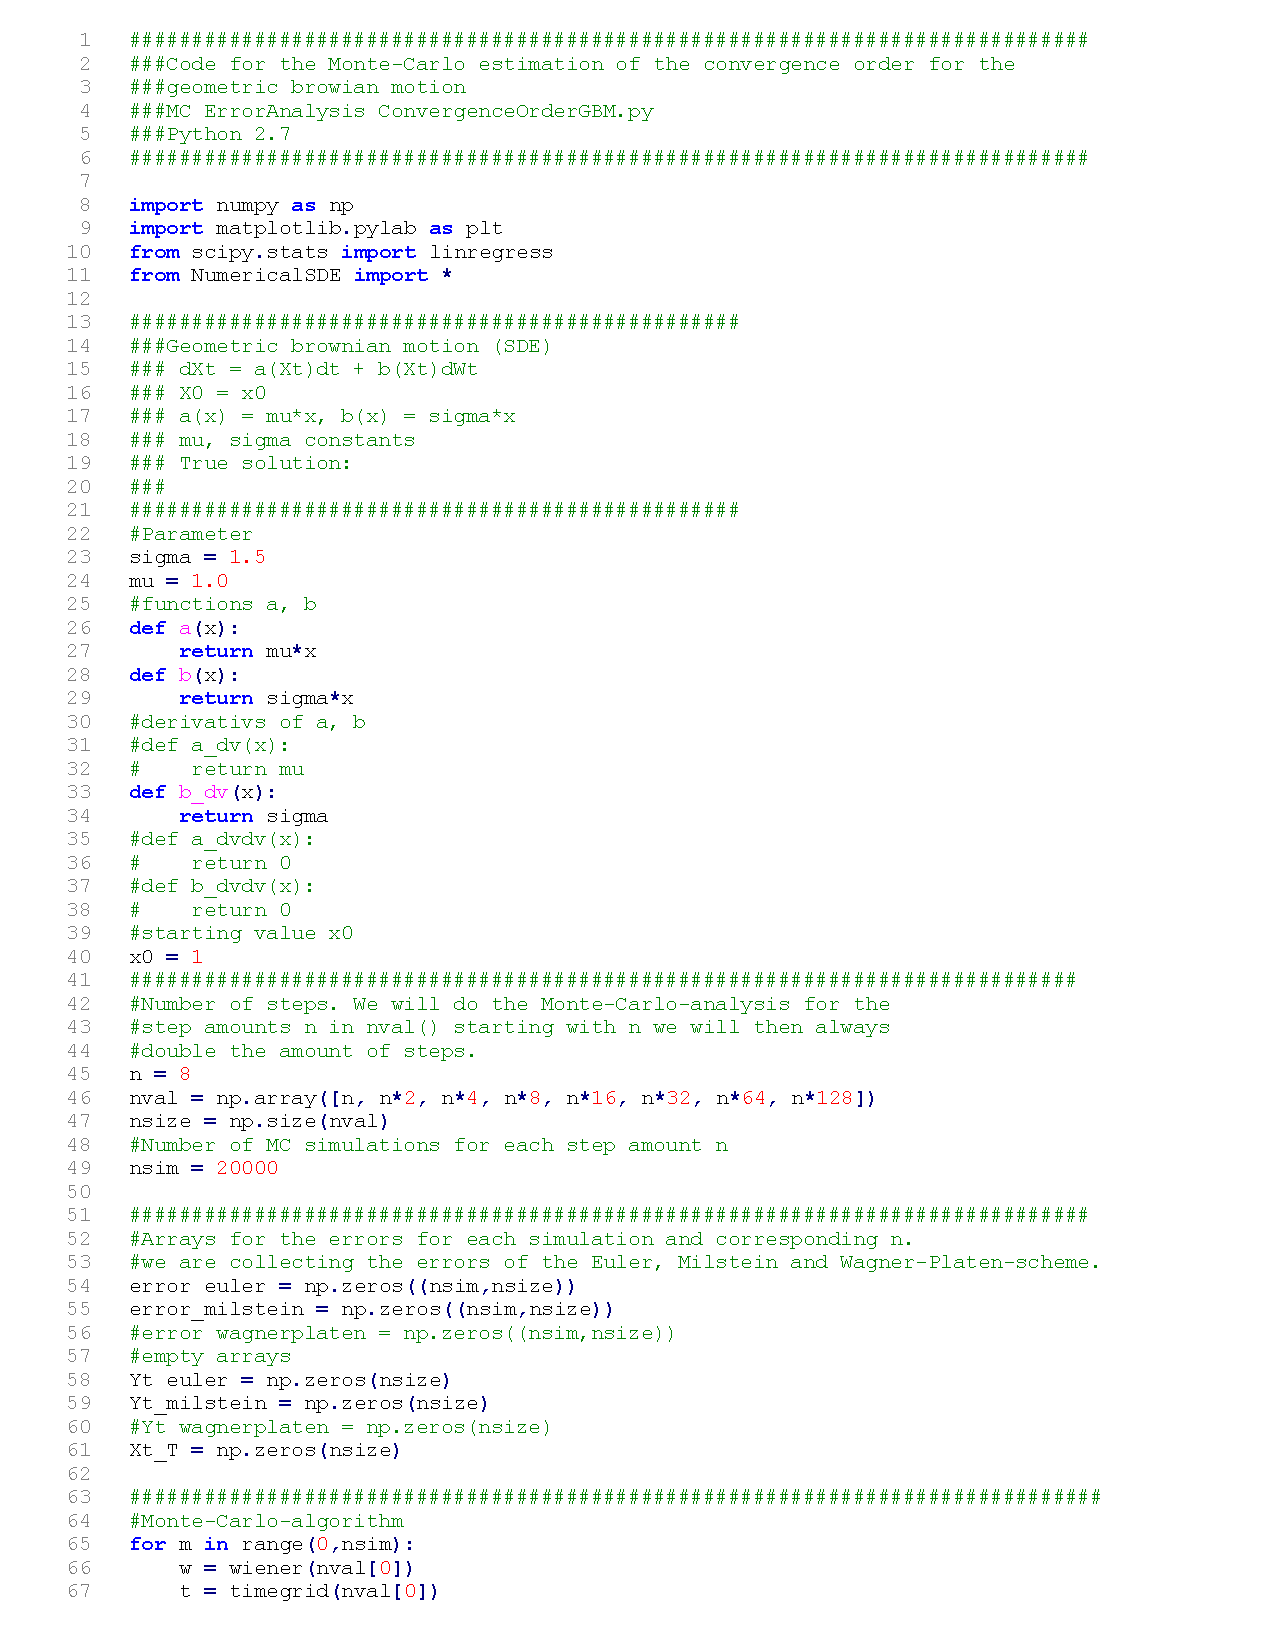
\includepdf[pages={-}]{Content/Code/MC_ConvergenceOrderGBM.pdf}
%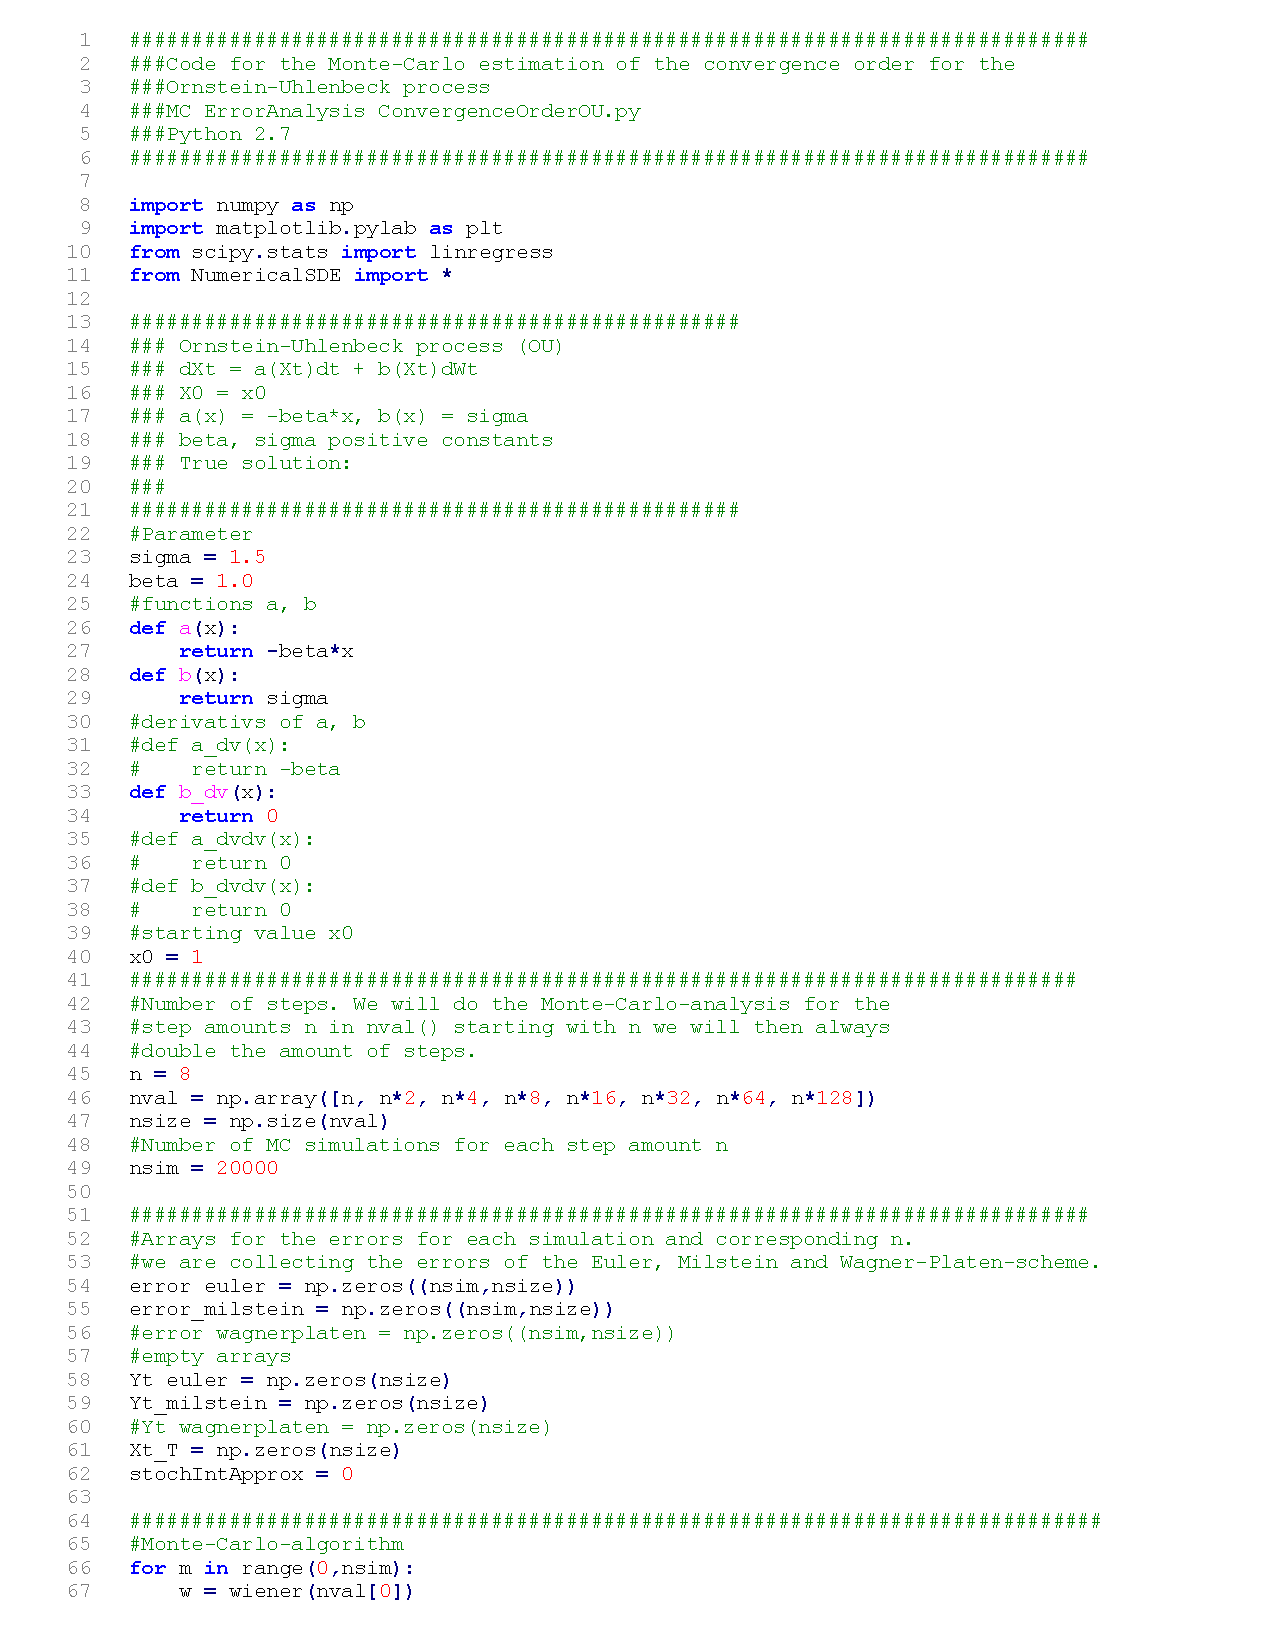
\includepdf[pages={-}]{Content/Code/MC_ConvergenceOrderOU.pdf}


\chapter{Additional plots}
\label{Graphics}
We included some additional figures in the next pages to illustrate the approximation schemes. Especially we also added some graphics of the Wagner-Platen approximation and its error-analysis. It has strong order 1.5. This scheme has not beed discussed in the main text of the thesis. However we implemented this scheme as well.


\begin{figure}[!h]
\centering
   \begin{subfigure}{0.49\linewidth} \centering
     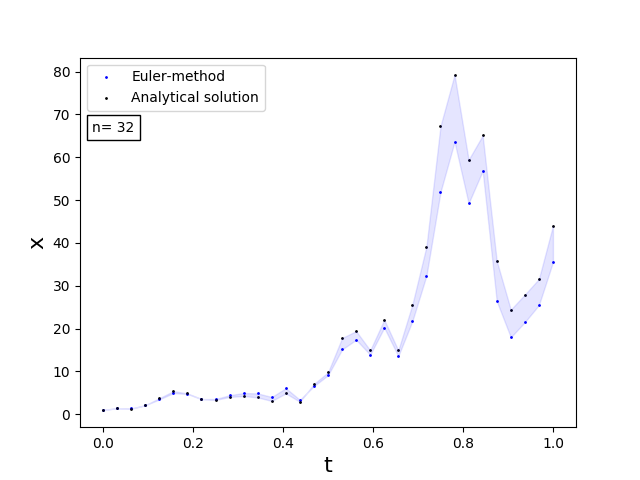
\includegraphics[scale=0.4]{Content/Graphics/Appendix/1gbm}
   \end{subfigure}
   \begin{subfigure}{0.49\linewidth} \centering
     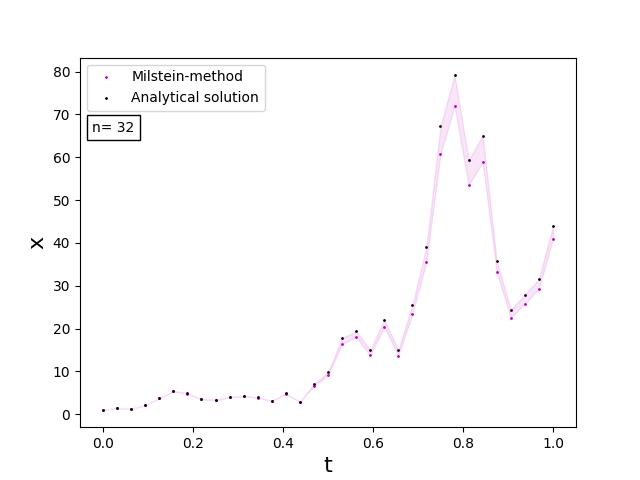
\includegraphics[scale=0.4]{Content/Graphics/Appendix/2gbm}
   \end{subfigure}
   \begin{subfigure}{0.49\linewidth} \centering
     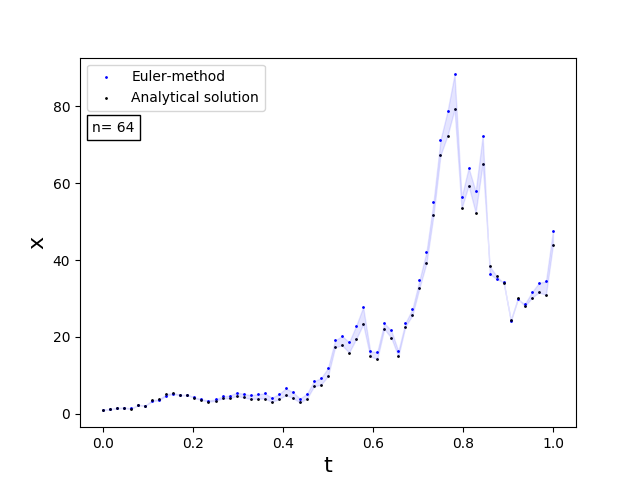
\includegraphics[scale=0.4]{Content/Graphics/Appendix/3gbm}
   \end{subfigure}
   \begin{subfigure}{0.49\linewidth} \centering
     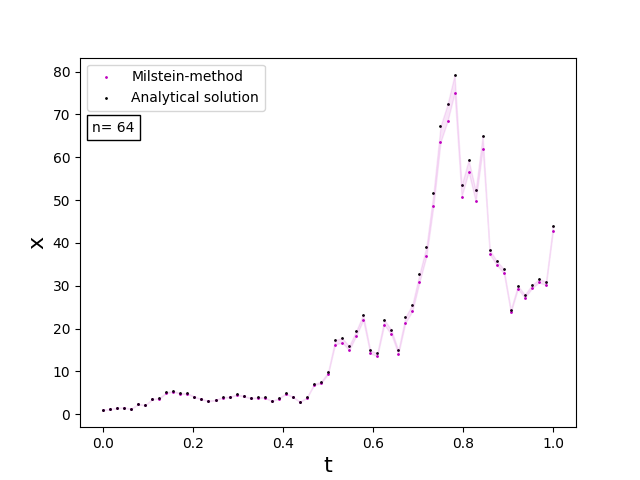
\includegraphics[scale=0.4]{Content/Graphics/Appendix/4gbm}
   \end{subfigure}
   \begin{subfigure}{0.49\linewidth} \centering
     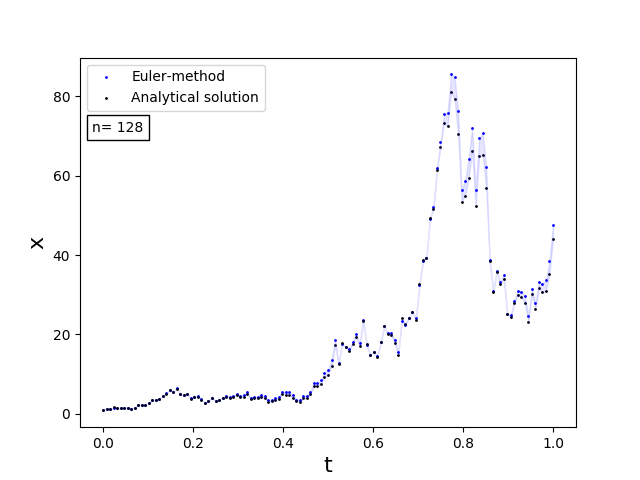
\includegraphics[scale=0.4]{Content/Graphics/Appendix/5gbm}
   \end{subfigure}
   \begin{subfigure}{0.49\linewidth} \centering
     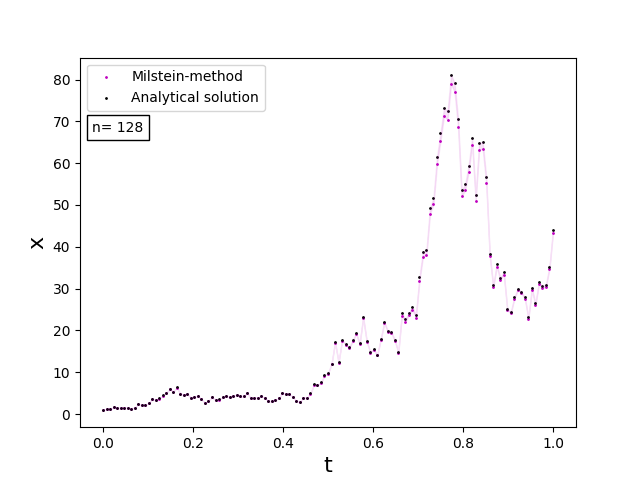
\includegraphics[scale=0.4]{Content/Graphics/Appendix/6gbm}
   \end{subfigure}
\caption{Approximation (colored dots) of the sample path of the geometric Brownian motion and the true sample path (black dots) for n = 32, 64, 128 using Euler and Milstein.}
\end{figure}

\begin{figure}[!h]
\centering
   \begin{subfigure}{0.49\linewidth} \centering
     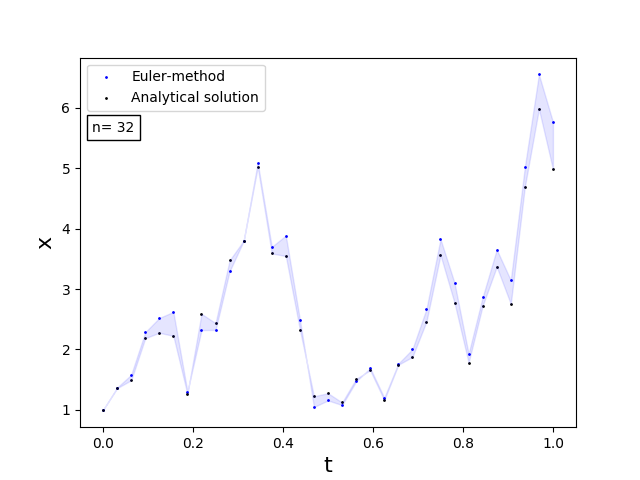
\includegraphics[scale=0.4]{Content/Graphics/Appendix/1gbm2}
   \end{subfigure}
   \begin{subfigure}{0.49\linewidth} \centering
     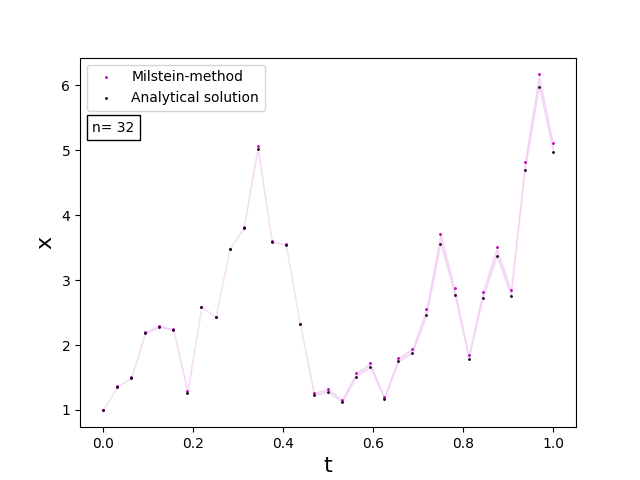
\includegraphics[scale=0.4]{Content/Graphics/Appendix/2gbm2}
   \end{subfigure}
   \begin{subfigure}{0.49\linewidth} \centering
     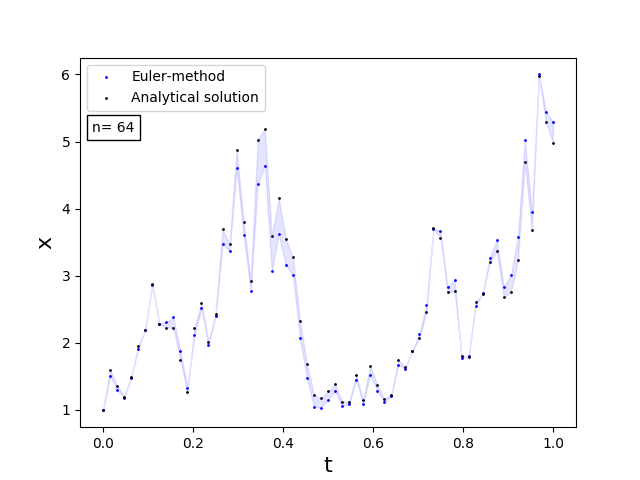
\includegraphics[scale=0.4]{Content/Graphics/Appendix/3gbm2}
   \end{subfigure}
   \begin{subfigure}{0.49\linewidth} \centering
     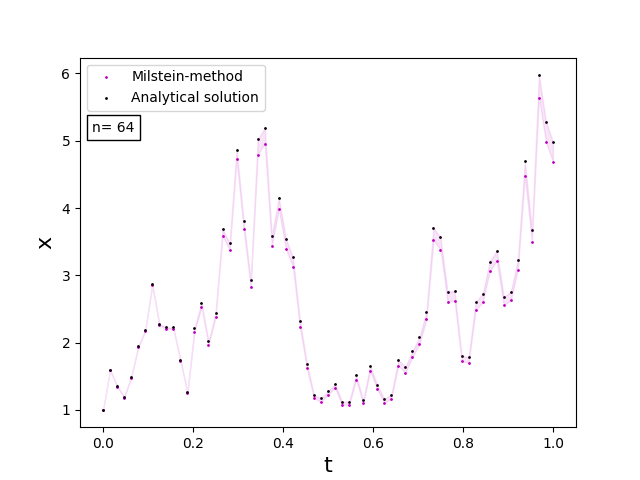
\includegraphics[scale=0.4]{Content/Graphics/Appendix/4gbm2}
   \end{subfigure}
   \begin{subfigure}{0.49\linewidth} \centering
     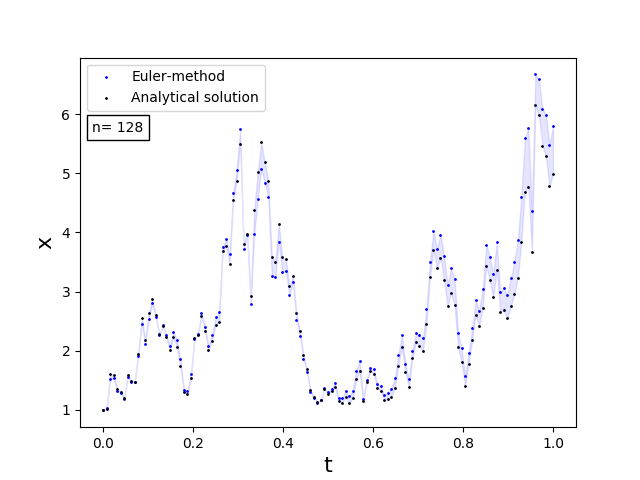
\includegraphics[scale=0.4]{Content/Graphics/Appendix/5gbm2}
   \end{subfigure}
   \begin{subfigure}{0.49\linewidth} \centering
     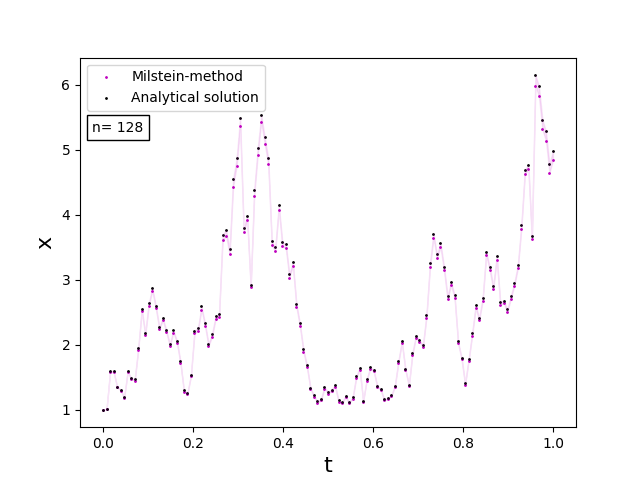
\includegraphics[scale=0.4]{Content/Graphics/Appendix/6gbm2}
   \end{subfigure}
\caption{Approximation (colored dots) of the sample path of the geometric Brownian motion and the true sample path (black dots) for n = 32, 64, 128 using Euler and Milstein.}
\end{figure}


\begin{figure}[!h]
\centering
   \begin{subfigure}{0.49\linewidth} \centering
     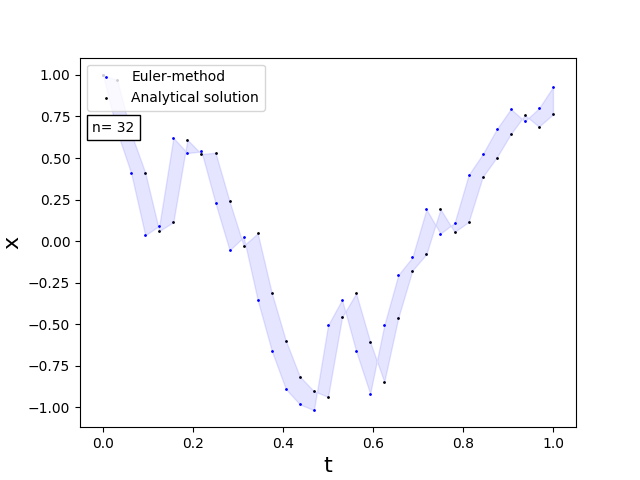
\includegraphics[scale=0.4]{Content/Graphics/Appendix/1ou}
   \end{subfigure}
   \begin{subfigure}{0.49\linewidth} \centering
     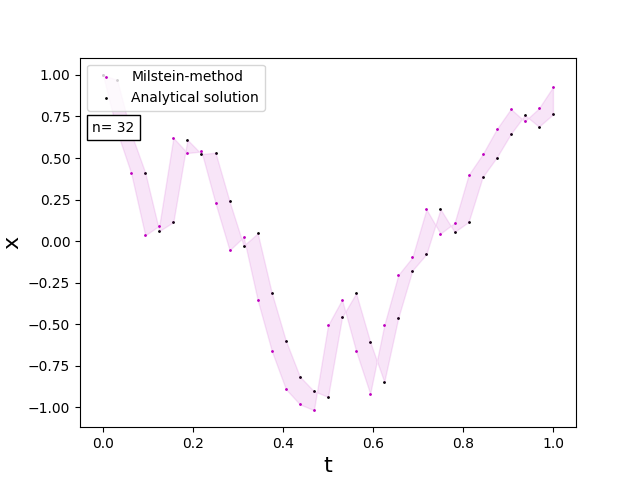
\includegraphics[scale=0.4]{Content/Graphics/Appendix/2ou}
   \end{subfigure}
   \begin{subfigure}{0.49\linewidth} \centering
     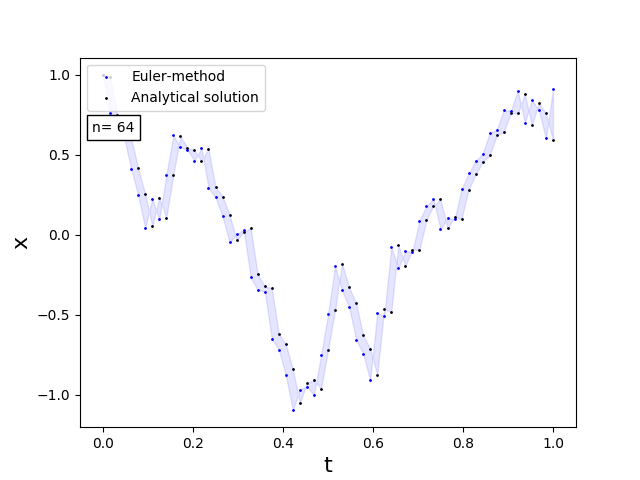
\includegraphics[scale=0.4]{Content/Graphics/Appendix/3ou}
   \end{subfigure}
   \begin{subfigure}{0.49\linewidth} \centering
     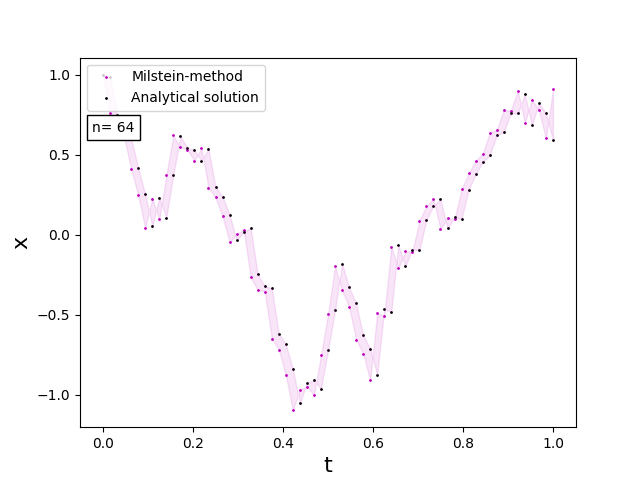
\includegraphics[scale=0.4]{Content/Graphics/Appendix/4ou}
   \end{subfigure}
   \begin{subfigure}{0.49\linewidth} \centering
     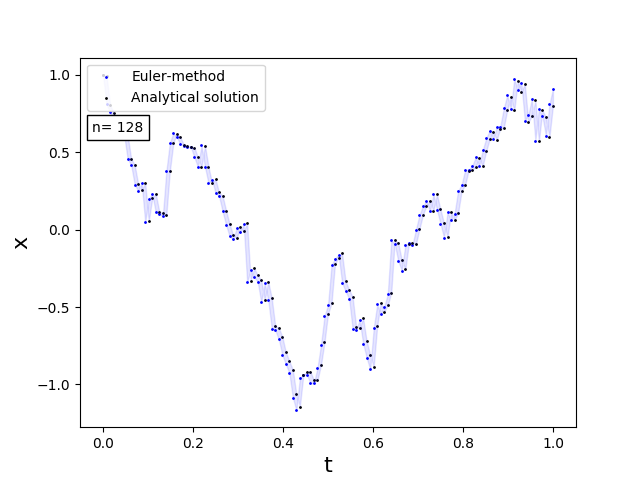
\includegraphics[scale=0.4]{Content/Graphics/Appendix/5ou}
   \end{subfigure}
   \begin{subfigure}{0.49\linewidth} \centering
     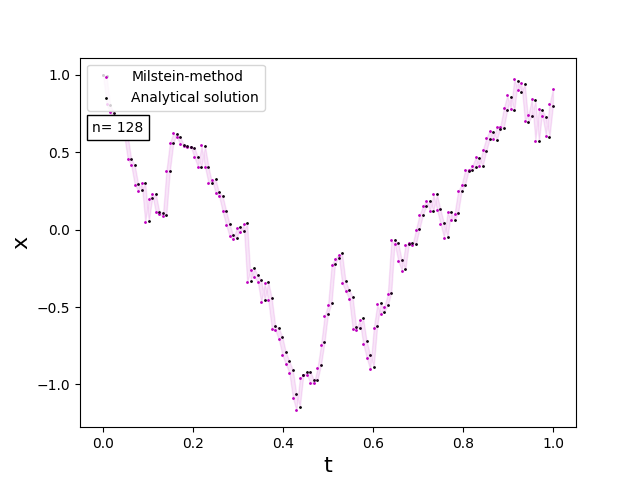
\includegraphics[scale=0.4]{Content/Graphics/Appendix/6ou}
   \end{subfigure}
\caption{Approximation (colored dots) of the sample path of the Ornstein-Uhlenbeck process and the true sample path (black dots) for n = 32, 64, 128 using Euler and Milstein.}
\end{figure}


\begin{figure}[!h]
\centering
   \begin{subfigure}{0.49\linewidth} \centering
     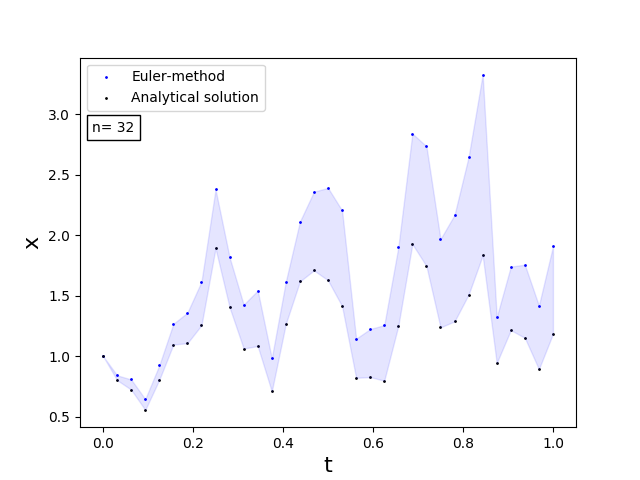
\includegraphics[scale=0.4]{Content/Graphics/Appendix/1gbm3}
   \end{subfigure}
   \begin{subfigure}{0.49\linewidth} \centering
     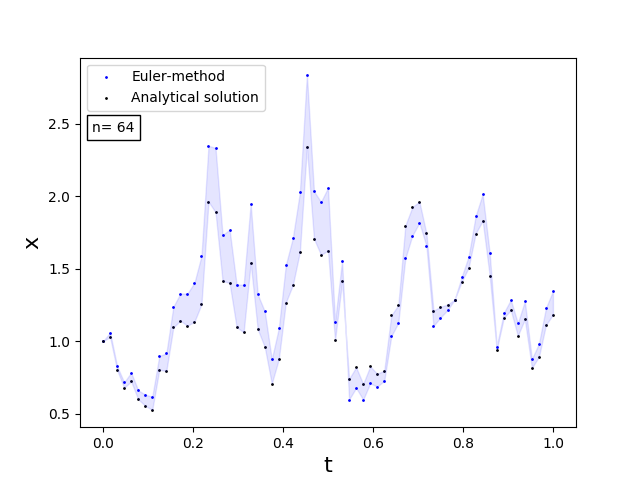
\includegraphics[scale=0.4]{Content/Graphics/Appendix/4gbm3}
   \end{subfigure}
   \begin{subfigure}{0.49\linewidth} \centering
     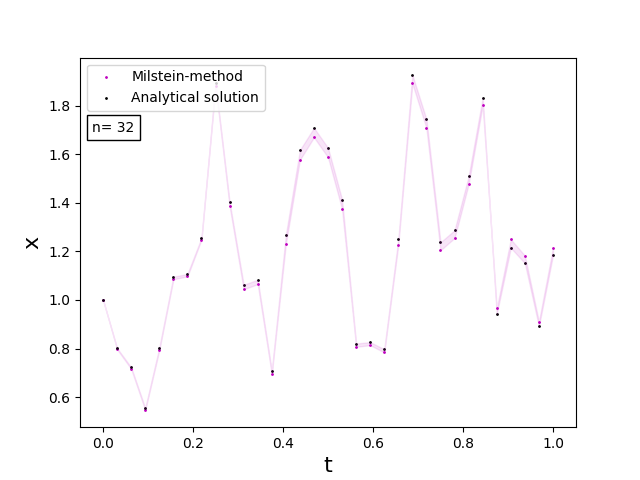
\includegraphics[scale=0.4]{Content/Graphics/Appendix/2gbm3}
   \end{subfigure}
   \begin{subfigure}{0.49\linewidth} \centering
     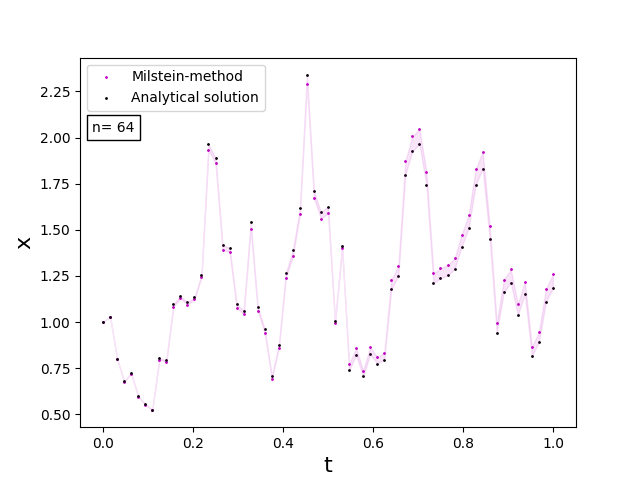
\includegraphics[scale=0.4]{Content/Graphics/Appendix/5gbm3}
   \end{subfigure}
   \begin{subfigure}{0.49\linewidth} \centering
     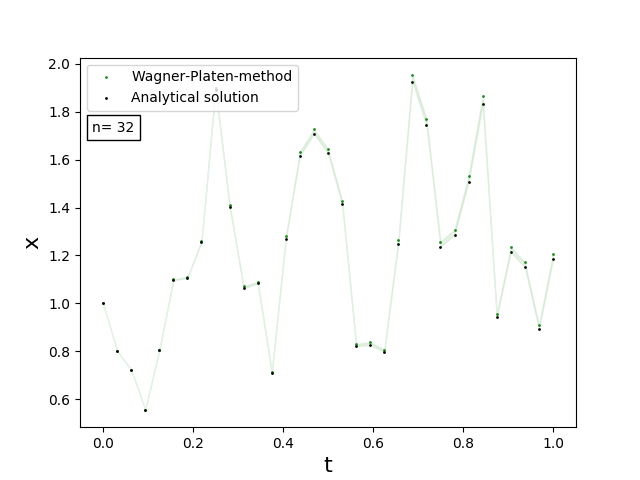
\includegraphics[scale=0.4]{Content/Graphics/Appendix/3gbm3}
   \end{subfigure}
   \begin{subfigure}{0.49\linewidth} \centering
     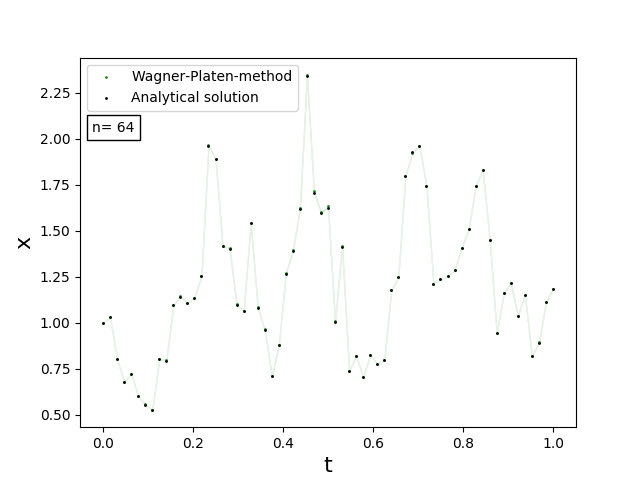
\includegraphics[scale=0.4]{Content/Graphics/Appendix/6gbm3}
   \end{subfigure}
\caption{Approximation (colored dots) of the sample path of the Ornstein-Uhlenbeck process and the true sample path (black dots) for n = 32, 64 using Euler, Milstein and Wagner-Platen.}
\end{figure}


\begin{figure}[!h]
     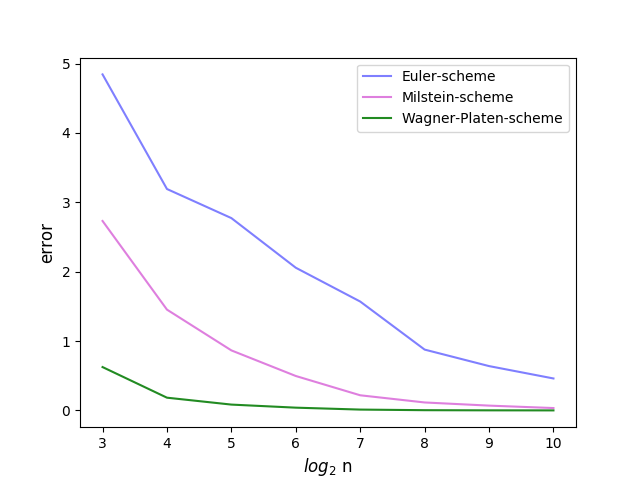
\includegraphics[scale=0.7]{Content/Graphics/Appendix/Error_analysis_gbm}
	\caption{Monte-Carlo estimates of the approximation error and the step amount n (logarithmized) for the geometric Brownian motion using Euler, Milstein, Wagner-Platen (20'000 simulations).}
\end{figure}
\begin{figure}[!h]
     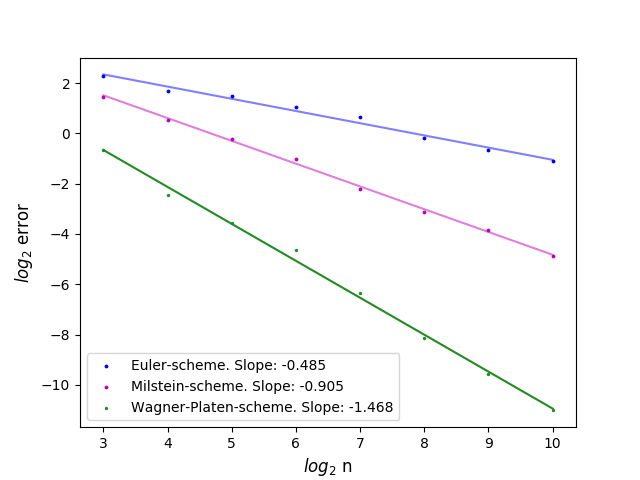
\includegraphics[scale=0.7]{Content/Graphics/Appendix/Conv_order_gbm}
\caption{Log-log plot of the approximation error and the step amount n for the geometric Brownian motion using Euler, Milstein, Wagner-Platen (20'000 simulations).} 
\end{figure}
